\documentclass{beamer}
\usepackage[utf8]{inputenc}

\usetheme{Madrid}
\usecolortheme{default}
\usepackage{amsmath,amssymb,amsfonts,amsthm}
\usepackage{mathtools}
\usepackage{txfonts}
\usepackage{tkz-euclide}
\usepackage{listings}
\usepackage{adjustbox}
\usepackage{array}
\usepackage{gensymb}
\usepackage{tabularx}
\usepackage{gvv}
\usepackage{lmodern}
\usepackage{circuitikz}
\usepackage{tikz}
\usepackage{graphicx}

\setbeamertemplate{page number in head/foot}[totalframenumber]

\usepackage{tcolorbox}
\tcbuselibrary{minted,breakable,xparse,skins}



\definecolor{bg}{gray}{0.95}
\DeclareTCBListing{mintedbox}{O{}m!O{}}{%
  breakable=true,
  listing engine=minted,
  listing only,
  minted language=#2,
  minted style=default,
  minted options={%
    linenos,
    gobble=0,
    breaklines=true,
    breakafter=,,
    fontsize=\small,
    numbersep=8pt,
    #1},
  boxsep=0pt,
  left skip=0pt,
  right skip=0pt,
  left=25pt,
  right=0pt,
  top=3pt,
  bottom=3pt,
  arc=5pt,
  leftrule=0pt,
  rightrule=0pt,
  bottomrule=2pt,
  toprule=2pt,
  colback=bg,
  colframe=orange!70,
  enhanced,
  overlay={%
    \begin{tcbclipinterior}
    \fill[orange!20!white] (frame.south west) rectangle ([xshift=20pt]frame.north west);
    \end{tcbclipinterior}},
  #3,
}
\lstset{
    language=C,
    basicstyle=\ttfamily\small,
    keywordstyle=\color{blue},
    stringstyle=\color{orange},
    commentstyle=\color{green!60!black},
    numbers=left,
    numberstyle=\tiny\color{gray},
    breaklines=true,
    showstringspaces=false,
}
%------------------------------------------------------------
%This block of code defines the information to appear in the
%Title page
\title %optional
{2.7.18}
\date{september 10,2025}
%\subtitle{A short story}

\author % (optional)
{EE25BTECH11006 - ADUDOTLA SRIVIDYA}

\begin{document}

\frame{\titlepage}

% ---------------- QUESTION ----------------
\begin{frame}{Question}
Vertices of a $\triangle ABC$ are $\vec{A}(4,6)$, $\vec{B}(1,5)$ and $\vec{C}(7,2)$.  
A line segment $DE$ is drawn intersecting AB and AC at D and E respectively such that  
$\dfrac{AD}{AB} = \dfrac{AE}{AC} = \dfrac{1}{3}$.  
Calculate the area of $\triangle ADE$ and compare it with the area of $\triangle ABC$.
\end{frame}

% ---------------- FORMULA ----------------
\begin{frame}{Formula}
\begin{itemize}
    \item Section formula for a point $P$ dividing $A$ and $B$ in ratio $m:n$:
    $
    \vec{P} = \frac{m\vec{B}+n\vec{A}}{m+n}
    $
    \item Area of triangle given 3 points $P,Q,R$:
    $
    \text{Area} = \frac{1}{2}\left| 
    (Q_x-P_x)(R_y-P_y) - (Q_y-P_y)(R_x-P_x)
    \right|
    $
\end{itemize}
\end{frame}

% ---------------- SOLUTION ----------------
\begin{frame}{Solution}
Let $A(4,6), B(1,5), C(7,2)$.
\begin{align}
D = \frac{1\cdot B + 2\cdot A}{1+2}
= \frac{1}{3}\begin{bmatrix}1+8 \\ 5+12 \end{bmatrix}
= \myvec{3\\\tfrac{17}{3}}
\end{align}

\begin{align}
E = \frac{1\cdot C + 2\cdot A}{1+2}
= \frac{1}{3}\begin{bmatrix}7+8 \\ 2+12 \end{bmatrix}
= \myvec{5\\\tfrac{14}{3}}
\end{align}
\end{frame}

\begin{frame}{Areas}
\begin{align}
\text{ar}(\Delta ABC) = \tfrac{1}{2}\left|
(1-4)(2-6) - (5-6)(7-4) \right| = \dfrac{15}{2}
\end{align}

\begin{align}
\text{ar}(\Delta ADE) = \tfrac{1}{2}\left|
(3-4)\brak{\tfrac{14}{3}-6} - \brak{\tfrac{17}{3}-6}(5-4) \right| = \dfrac{5}{6}
\end{align}
\begin{align}
\frac{\text{ar}(\Delta ADE)}{\text{ar}(\Delta ABC)} = \frac{1}{9}
\end{align}
\end{frame}

% ---------------- PURE PYTHON ----------------
\begin{frame}[fragile]{Pure Python Plot (Part 1)}
\begin{lstlisting}[language=Python]
import numpy as np
import matplotlib.pyplot as plt

A = np.array([4, 6])
B = np.array([1, 5])
C = np.array([7, 2])

# Points D and E using section formula (1:2)
D = (2*A + B)/3
E = (2*A + C)/3
\end{lstlisting}
\end{frame}

\begin{frame}[fragile]{Pure Python Plot (Part 2)}
\begin{lstlisting}[language=Python]
def area(P, Q, R):
    return 0.5 * np.linalg.norm(np.linalg.det(np.array([
        [Q[0] - P[0], R[0] - P[0]],
        [Q[1] - P[1], R[1] - P[1]]
    ])))

area_ABC = area(A, B, C)
area_ADE = area(A, D, E)
ratio = area_ADE / area_ABC
print("Ratio =", ratio)
\end{lstlisting}
\end{frame}

\begin{frame}[fragile]{Pure Python Plot (Part 3)}
\begin{lstlisting}[language=Python]
plt.plot([A[0], B[0], C[0], A[0]],
         [A[1], B[1], C[1], A[1]], 'k-', label='ΔABC')
plt.plot([A[0], D[0], E[0], A[0]],
         [A[1], D[1], E[1], A[1]], 'r--', label='ΔADE')

points = np.vstack([A,B,C,D,E])
labels = ['A(4,6)','B(1,5)','C(7,2)','D(3,17/3)','E(5,14/3)']
plt.scatter(points[:,0], points[:,1], color='black')
for i, txt in enumerate(labels):
    plt.annotate(txt, (points[i,0], points[i,1]),
                 textcoords="offset points", xytext=(0,10), ha='center')

plt.xlabel('$x$'); plt.ylabel('$y$')
plt.legend(); plt.grid(True); plt.axis('equal')
plt.savefig('figs/fig2_7_18.png')
plt.show()
\end{lstlisting}
\end{frame}

% ---------------- C CODE ----------------
\begin{frame}[fragile]{C Code: formula.c}
\begin{lstlisting}[language=C]
#include <stdio.h>

// Section formula for point dividing AB in ratio m:n
void section_formula(float *P, float *A, float *B, int m, int n, int k){
    for (int i = 0; i < k ; i++) {
        P[i] = (m*B[i] + n*A[i])/(m+n);
    }
}

// Area of triangle given 3 points
float triangle_area(float *A, float *B, float *C){
    float det = (B[0]-A[0])*(C[1]-A[1]) - (B[1]-A[1])*(C[0]-A[0]);
    if(det < 0) det = -det;
    return 0.5f * det;
}
\end{lstlisting}
\end{frame}

% ---------------- CPYTHON ----------------
\begin{frame}[fragile]{Python + Ctypes (cpython.py, Part 1)}
\begin{lstlisting}[language=Python]
import ctypes, numpy as np, matplotlib.pyplot as plt, os

c_lib = ctypes.CDLL('./formula.so')

c_lib.section_formula.argtypes = [
    ctypes.POINTER(ctypes.c_float),
    ctypes.POINTER(ctypes.c_float),
    ctypes.POINTER(ctypes.c_float),
    ctypes.c_int, ctypes.c_int, ctypes.c_int
]
c_lib.section_formula.restype = None

c_lib.triangle_area.argtypes = [
    ctypes.POINTER(ctypes.c_float),
    ctypes.POINTER(ctypes.c_float),
    ctypes.POINTER(ctypes.c_float)
]
c_lib.triangle_area.restype = ctypes.c_float
\end{lstlisting}
\end{frame}

\begin{frame}[fragile]{Python + Ctypes (cpython.py, Part 2)}
\begin{lstlisting}[language=Python]
A = np.array([4, 6], dtype=np.float32)
B = np.array([1, 5], dtype=np.float32)
C = np.array([7, 2], dtype=np.float32)

D, E = np.zeros(2, dtype=np.float32), np.zeros(2, dtype=np.float32)

c_lib.section_formula(D.ctypes.data_as(ctypes.POINTER(ctypes.c_float)),
    A.ctypes.data_as(ctypes.POINTER(ctypes.c_float)),
    B.ctypes.data_as(ctypes.POINTER(ctypes.c_float)), 1, 2, 2)

c_lib.section_formula(E.ctypes.data_as(ctypes.POINTER(ctypes.c_float)),
    A.ctypes.data_as(ctypes.POINTER(ctypes.c_float)),
    C.ctypes.data_as(ctypes.POINTER(ctypes.c_float)), 1, 2, 2)

area_ABC = c_lib.triangle_area(A.ctypes.data_as(ctypes.POINTER(ctypes.c_float)),
    B.ctypes.data_as(ctypes.POINTER(ctypes.c_float)),
    C.ctypes.data_as(ctypes.POINTER(ctypes.c_float)))

area_ADE = c_lib.triangle_area(A.ctypes.data_as(ctypes.POINTER(ctypes.c_float)),
    D.ctypes.data_as(ctypes.POINTER(ctypes.c_float)),
    E.ctypes.data_as(ctypes.POINTER(ctypes.c_float)))
\end{lstlisting}
\end{frame}

\begin{frame}[fragile]{Python + Ctypes (cpython.py, Part 3)}
\begin{lstlisting}[language=Python]
ratio = area_ADE / area_ABC

print("A =", A, "B =", B, "C =", C)
print("D =", D, "E =", E)
print("Areas: ABC =", area_ABC, " ADE =", area_ADE)
print("Ratio =", ratio)

# Plot
os.makedirs("figs", exist_ok=True)
plt.plot([A[0], B[0], C[0], A[0]],[A[1], B[1], C[1], A[1]],'b-',label="ΔABC")
plt.plot([A[0], D[0], E[0], A[0]],[A[1], D[1], E[1], A[1]],'r--',label="ΔADE")
plt.legend(); plt.grid(True); plt.axis('equal')
plt.savefig("figs/fig_cpython_2_7_18.png")
plt.show()
\end{lstlisting}
\end{frame}

\begin{frame}{Plot}
\centering
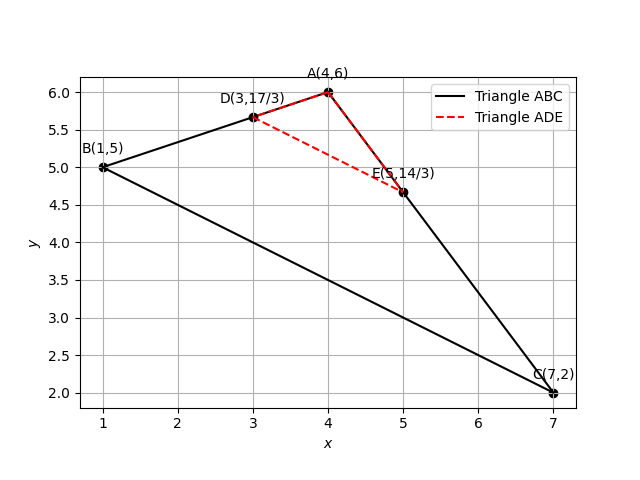
\includegraphics[width=0.6\linewidth]{figs/fig4.png}
\caption{Internal Division: ΔADE inside ΔABC}
\end{frame}

\end{document}
